\input{"Blatt1header.tex"}

\title{Übung 1: Graphische Auswertung}
\author{Joris Daus \and Vincent Wirsdörfer}
\date{17.10.2023}

\begin{document}
\maketitle
    	\section{Graphische Darstellung}
            Das Experiment soll die Abstandsabhängigkeit von radioaktivem Zerfall beschreiben.
            Dabei ist $d [\unit{\centi\meter}]$ die Dicke des abschirmenden Bleis. $N$ ist die Anzahl an 
            Gamma-Quanten, die in $t = 60 \unit{\second}$ gezählt wurden.
%           
        \begin{figure}%{0.48\textwidth}
                \centering
                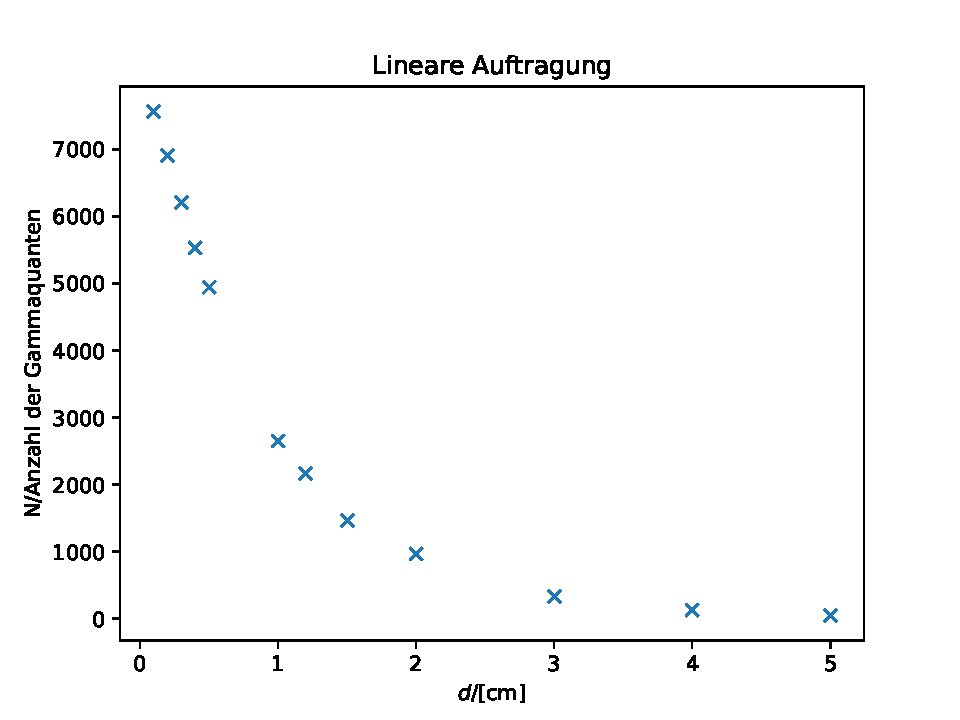
\includegraphics{Auswertung_linear}
                \label{fig:lin}
                \caption{lineare Auftragung}
        \end{figure}
%
        \begin{figure}%{0.48\textwidth}
                \centering
                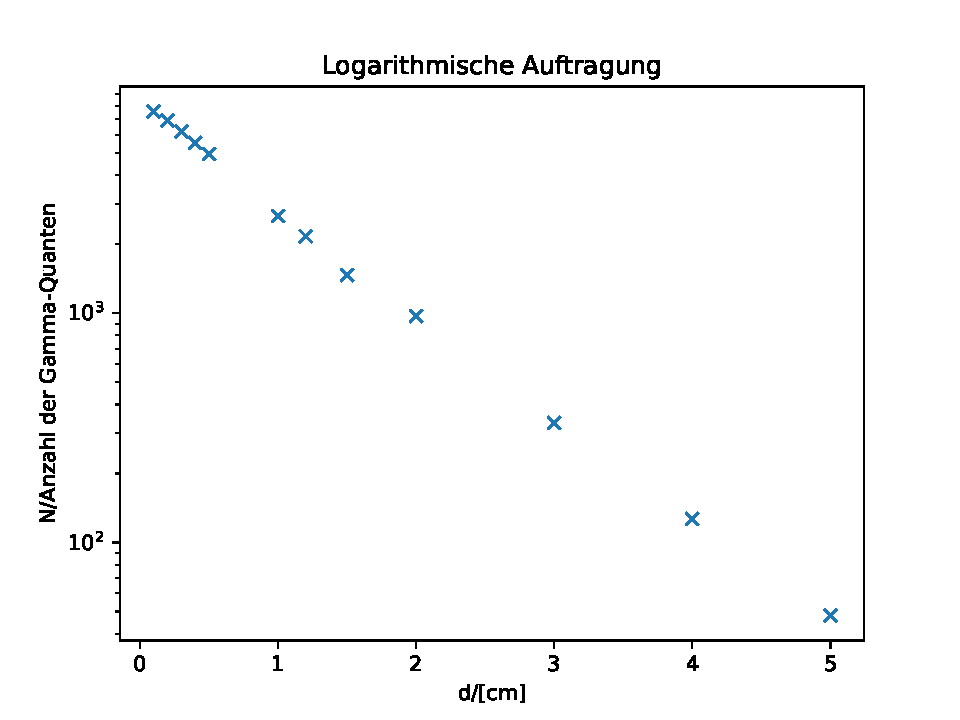
\includegraphics{Auswertung_log}
                \label{fig:log}
                \caption{logarithmische Auftragung}    
        \end{figure}
%
\end{document}